\section{再生关系}
\label{sec:rkhs-reproducing-relation}

上一节得到候选空间的两项要求：元素是真正的函数，每个点的读取随函数连续变化。把这两项要求作为定义，就得到本章的空间。

全章的数域记为$\mathbb K$，取$\mathbb R$或$\mathbb C$。复内积沿用全书的约定：$\langle f,g\rangle$对第一个变量共轭线性、对第二个变量线性。主线中的例子都是实值函数，此时共轭不起作用；保留复数情形，是为了第~\ref{sec:rkhs-mercer}节使用复Hilbert空间上的谱定理时不必另行改写。

\begin{definition}[再生核Hilbert空间]
\label{def:rkhs-rkhs}
设$X$是非空集合，$H$是由函数$f:X\to\mathbb K$组成的Hilbert空间，其加法与数乘按逐点方式定义。对$x\in X$，称$\delta_x:H\to\mathbb K$，$\delta_x(f)=f(x)$为$x$处的\term{点评估泛函}（evaluation functional）。若对每个$x\in X$，$\delta_x$都是有界线性泛函，则称$H$为$X$上的\term{再生核Hilbert空间}（reproducing kernel Hilbert space），简称RKHS。
\end{definition}

定义中有两个条件。逐点运算这一条保证$H$的零元就是处处为零的函数，因而“两个元素相等”与“两个函数在每一点取值相同”是同一件事；$L^2$的元素是函数类，不在这个定义的讨论范围内。

有界性一条就是上一节的要求~\eqref{eq:rkhs-stability-requirement}：$\delta_x$线性且有界，等价于存在$C_x$使$\lvert f(x)\rvert\leq C_x\lVert f\rVert_H$，把$f$换成$f-g$就得到要求的不等式。定义只要求每个点各有一个常数$C_x$，不要求这些常数有共同上界。是否存在统一的常数，下文会由核在对角线上的取值读出。

\subsection{点评估界}
\label{sec:rkhs-evaluation-bounds}

判断一个函数空间是不是RKHS，关键是对每个$x$估计$\lvert f(x)\rvert/\lVert f\rVert_H$。先看有限维空间，再看一个无限维空间。

\paragraph{仿射函数空间}

设$X=\mathbb R$，令$H_{\mathrm{aff}}$为仿射函数$f(t)=a+bt$全体，内积取系数向量的内积：
\[
\langle a+bt,\ a'+b't\rangle=\overline a\,a'+\overline b\,b' .
\]
系数$(a,b)$与函数一一对应，所以$H_{\mathrm{aff}}$与$\mathbb K^2$等距同构，是二维Hilbert空间。

对固定的$x$，函数值是系数向量$(a,b)$与$(1,x)$的内积，由Cauchy--Schwarz不等式，
\[
\lvert f(x)\rvert=\lvert a\cdot1+b\cdot x\rvert\leq\sqrt{1+x^2}\,\lVert f\rVert .
\]
因此每个点评估都有界，$H_{\mathrm{aff}}$是RKHS。常数$\sqrt{1+x^2}$随$\lvert x\rvert$增大而无界，在整条实轴上没有统一的常数；若把定义域限制为$[-1,1]$，统一常数是$\sqrt2$。

同样的计算适用于次数不超过$m$的多项式空间，只是常数变为$(\sum_{k\leq m}\lvert x\rvert^{2k})^{1/2}$。更一般地，任何有限维函数空间配上任何内积都是RKHS，因为有限维赋范空间上的线性泛函都有界。点评估界真正需要论证的是无限维的情形。

\paragraph{左端固定的一阶Sobolev函数}

取$X=[0,1]$，令$H_{\min}$为$H^1(0,1)$中满足$f(0)=0$的实值函数全体，每个元素取其绝对连续代表，内积只用导数：
\[
\langle f,g\rangle_{H_{\min}}=\int_0^1f'(t)\,g'(t)\,\mathrm dt .
\]
先核对这是内积。若$\langle f,f\rangle=0$，则$f'=0$几乎处处，绝对连续性给出$f(x)=f(0)+\int_0^xf'=0$。这里由$f(0)=0$排除了常数函数，导数的$L^2$范数才能成为范数。

再核对完备性。映射$f\mapsto f'$把$H_{\min}$映到$L^2(0,1)$，保持内积。反过来，对任意$g\in L^2(0,1)$，函数$x\mapsto\int_0^xg$绝对连续，左端为零，导数几乎处处等于$g$，所以这个映射是满射。因此$H_{\min}$与$L^2(0,1)$等距同构，它继承了完备性，是无限维Hilbert空间。

点评估界来自同一个积分表示。对$x\in[0,1]$，把$f(x)$写成导数的累计，再用Cauchy--Schwarz不等式：
\begin{equation}
\lvert f(x)\rvert=\Bigl\lvert\int_0^xf'(t)\,\mathrm dt\Bigr\rvert
\leq\sqrt x\,\lVert f\rVert_{H_{\min}} .
\label{eq:rkhs-hmin-point-bound}
\end{equation}
所以$H_{\min}$是RKHS，统一常数为$1$。常数$\sqrt x$在$x=0$处为零，这与所有元素在左端取零相符：越靠近左端，函数积累变化的路程越短，读数越受控制。

这个例子说明了无限维空间中点评估受控的机制。范数控制的是导数的平方积分，而点值是导数沿一段路径的累计，Cauchy--Schwarz不等式把前者转化为后者的界。$L^2$范数只控制函数本身的平均大小，没有这样的转化，所以尖峰函数能逃脱控制。

\subsection{核截面}
\label{sec:rkhs-kernel-sections}

点评估界说明$\delta_x$是有界线性泛函。下一步要把读数写成内积。在进入无限维之前，先把有限维的情形算清楚，下面的每个结论在无限维都有对应。

\paragraph{有限维的样板：读坐标的向量}

设$\bm A$是$n\times n$实对称正定矩阵，在$\mathbb R^n$上取内积
\[
\langle\bm u,\bm v\rangle_{\bm A}=\bm u^{\top}\bm A\bm v .
\]
要读出第$i$个坐标$v_i$，用标准单位向量$\bm e_i$作内积并不奏效，那样读出的是$(\bm A\bm v)_i$。

我们需要一个向量$\bm w$，使下式对一切$\bm v$成立：
\[
\bm w^{\top}\bm A\bm v=v_i .
\]
这等价于$\bm A\bm w=\bm e_i$。记$\bm K=\bm A^{-1}$，所求向量就是$\bm K\bm e_i$，即$\bm K$的第$i$列，并且
\begin{equation}
v_i=\langle\bm K\bm e_i,\bm v\rangle_{\bm A}\qquad(\bm v\in\mathbb R^n).
\label{eq:rkhs-finite-reproducing}
\end{equation}
读取坐标的向量恰好是逆矩阵的列。把两列作内积，得到
\[
\langle\bm K\bm e_i,\bm K\bm e_j\rangle_{\bm A}=\bm K_{i,j} ,
\]
矩阵$\bm K$自身就是这些读坐标向量的Gram矩阵。

用具体的数算一遍。取三个下标对应$x=\tfrac13,\tfrac23,1$，令$\bm K_{i,j}=\min(x_i,x_j)$：
\[
\bm K=\frac13\begin{bmatrix}1&1&1\\1&2&2\\1&2&3\end{bmatrix},\qquad
\bm A=\bm K^{-1}=3\begin{bmatrix}2&-1&0\\-1&2&-1\\0&-1&1\end{bmatrix}.
\]
取向量$\bm v=(\tfrac89,\tfrac89,0)^{\top}$，先算$\bm A\bm v$：
\[
\bm A\bm v=(\tfrac83,\tfrac83,-\tfrac83)^{\top}.
\]
第二个坐标的读取向量是$\bm K$的第二列$(\tfrac13,\tfrac23,\tfrac23)^{\top}$，与$\bm A\bm v$作普通点积，
\[
\tfrac13\cdot\tfrac83+\tfrac23\cdot\tfrac83-\tfrac23\cdot\tfrac83=\tfrac89,
\]
恰好是$v_2$。

矩阵$\bm A$还有一个值得注意的含义。记$v_0=0$，$h=\tfrac13$，直接展开二次型，得到
\begin{equation}
\bm v^{\top}\bm A\bm v=\frac1h\sum_{i=1}^3(v_i-v_{i-1})^2 .
\label{eq:rkhs-finite-difference-form}
\end{equation}
右端正是差分形式的$\int_0^1f'(t)^2\,\mathrm dt$。所以这个$\bm K$与$H_{\min}$的内积有关，下面将看到它的连续版本。

\paragraph{再生关系与再生核}

现在回到一般的RKHS。第~\ref{chap:linear-functionals}章的Riesz表示定理指出：Hilbert空间上的每个有界线性泛函都唯一地写成与某个向量的内积，且泛函的范数等于该向量的长度。把它用于每个点评估，对每个$x\in X$就存在唯一的$K_x\in H$，使得
\begin{equation}
f(x)=\langle K_x,f\rangle_H\qquad(f\in H),
\label{eq:rkhs-reproducing}
\end{equation}
并且$\lVert\delta_x\rVert=\lVert K_x\rVert_H$。

这就是式~\eqref{eq:rkhs-finite-reproducing}的无限维版本：$K_x$是读取第$x$个坐标的向量。$K_x$本身是$H$中的元素，所以也是$X$上的函数。定义二元函数
\begin{equation}
K(y,x)=K_x(y)=\langle K_y,K_x\rangle_H\qquad(x,y\in X),
\label{eq:rkhs-kernel-definition}
\end{equation}
其中第二个等号是对$f=K_x$在点$y$处使用式~\eqref{eq:rkhs-reproducing}。称$K$为$H$的\term{再生核}（reproducing kernel），称$K_x=K(\cdot,x)$为核在$x$处的\term{核截面}（kernel section）。

式~\eqref{eq:rkhs-reproducing}称为\term{再生性质}（reproducing property）：在$x$处读取$f$，等于拿固定函数$K_x$与$f$作内积。把$f$换成另一个核截面，读出的又是核本身的值，“再生”一词即由此而来。表~\ref{tab:rkhs-dictionary}列出有限维与RKHS的对应，图~\ref{fig:rkhs-kernel-as-matrix}以最小值核为例画出从矩阵到二元函数的过渡。

\begin{BookInlineTable}
  \centering
  \begin{tabular}{@{}ll@{}}
    \toprule
    $\mathbb R^n$，内积矩阵$\bm A$ & RKHS $H$\\
    \midrule
    下标$i$ & 点$x\in X$\\
    坐标$v_i$ & 函数值$f(x)$\\
    读坐标的向量$\bm K\bm e_i$ & 核截面$K_x$\\
    $v_i=\langle\bm K\bm e_i,\bm v\rangle_{\bm A}$ & $f(x)=\langle K_x,f\rangle_H$\\
    矩阵元素$\bm K_{i,j}$ & 核值$K(x,y)$\\
    $\bm K$的第$j$列 & $K_y=K(\cdot,y)$\\
    $\bm K$半正定 & $K$是正定核\\
    \bottomrule
  \end{tabular}
  \caption{有限维内积空间与RKHS的对应。核是下标取遍$X\times X$的矩阵，核截面是它的列。}
  \label{tab:rkhs-dictionary}
\end{BookInlineTable}

\begin{BookInlineFigure}
  \centering
  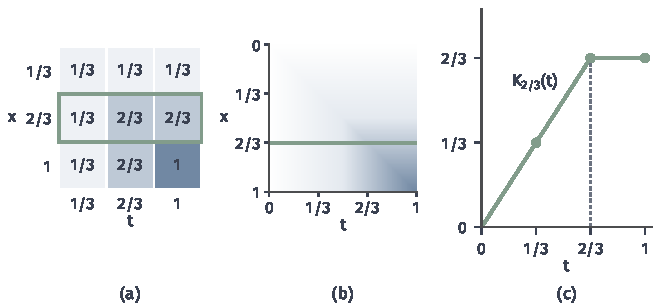
\includegraphics[width=112mm]{figures/04-spaces-measures-and-geometry/03-function-spaces/matplotlib/rkhs-kernel-as-matrix/figure.pdf}
  \caption{最小值核是一个连续下标的矩阵。(a)网格$\tfrac13,\tfrac23,1$上的矩阵$\bm K$，绿框是$x=\tfrac23$对应的行。(b)下标连成一片后的二元函数$\min(t,x)$，绿线是同一行。(c)沿绿线读出的函数就是核截面$K_{2/3}(t)=\min(t,\tfrac23)$，三个圆点是(a)中绿框内的三个数。}
  \label{fig:rkhs-kernel-as-matrix}
\end{BookInlineFigure}

类比有两处要留心。第一，有限维中$\bm K$与$\bm A$互逆，二者同样好用；无限维中通常只有$K$还是一个函数。式~\eqref{eq:rkhs-finite-difference-form}显示，网格加密时$\bm A$的元素以$1/h$的速度增长，它的极限不是二元函数，而是求导运算。所以无限维的内积一般不能用“矩阵元素”写出，我们只留下$K$。

第二，$\mathbb R^n$中每个向量都有有限长度，而函数空间中“有限长度”是实实在在的限制。$\mathbb K^X$中的绝大多数函数不属于$H$。核截面总在$H$中，标准单位向量的对应物，即只在$x$处有值的“尖峰”，却通常不在$H$中；这正是$L^2$上点值出问题的原因，读取坐标的向量在那里不存在。

\paragraph{两个例子中的核截面}

在$H_{\mathrm{aff}}$中，设$K_x=c+dt$，再生性质要求下式对一切$a,b$成立：
\[
\overline c\,a+\overline d\,b=a+bx .
\]
比较系数得$c=1$，$d=\overline x=x$。所以
\[
K_x(t)=1+xt,\qquad K(t,x)=1+tx ,
\]
称为仿射核。

图~\ref{fig:rkhs-reproducing-geometry}把这个计算画在系数平面上。核截面$K_x$对应向量$(1,x)$，读取$f=1+t$在$x=\tfrac12$处的值，就是计算$(1,1)$与$(1,\tfrac12)$的内积$1.5$。而$K_{-1}=(1,-1)$与$(1,1)$正交，对应$f(-1)=0$。函数在某点取零，几何上就是它与该点的核截面垂直。

\begin{BookInlineFigure}
  \centering
  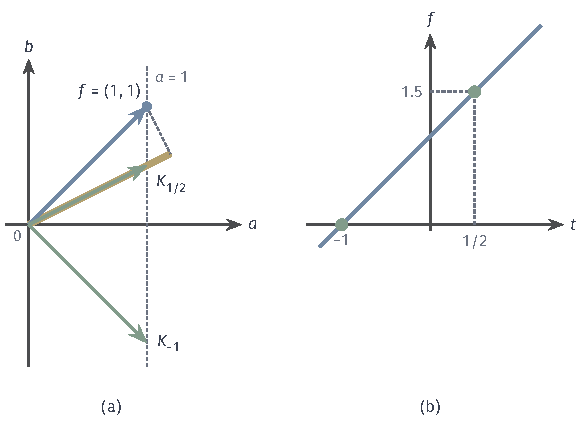
\includegraphics[width=99.4mm]{figures/04-spaces-measures-and-geometry/03-function-spaces/tikz/rkhs-reproducing-geometry/figure.pdf}
  \caption{仿射函数空间中再生性质的几何。(a)系数平面$(a,b)$与空间等距；蓝色向量是$f=1+t$，绿色向量是核截面$K_x=1+xt$，都落在虚线$a=1$上。黄色线段是$f$在$K_{1/2}$方向上的投影，其长度乘以$\lVert K_{1/2}\rVert$等于$f(1/2)=1.5$；$K_{-1}$与$f$垂直。(b)同一函数的图像，圆点标出$t=1/2$处的读数$1.5$与$t=-1$处的零点。}
  \label{fig:rkhs-reproducing-geometry}
\end{BookInlineFigure}

在$H_{\min}$中，式~\eqref{eq:rkhs-hmin-point-bound}的推导已经把$f(x)$写成了对$f'$的积分：
\[
f(x)=\int_0^1\mathbf 1_{[0,x]}(t)\,f'(t)\,\mathrm dt .
\]
只需找一个左端为零、导数为$\mathbf 1_{[0,x]}$的函数，它就是$K_x(t)=\min(t,x)$：在$[0,x]$上斜率为$1$，在$[x,1]$上保持常数$x$。

直接核对：
\[
\langle K_x,f\rangle_{H_{\min}}=\int_0^xf'(t)\,\mathrm dt=f(x) .
\]
称
\[
K(t,x)=\min(t,x)\qquad(t,x\in[0,1])
\]
为\term{最小值核}（minimum kernel）。它就是图~\ref{fig:rkhs-kernel-as-matrix}中的矩阵取遍全部下标的结果，式~\eqref{eq:rkhs-finite-difference-form}也随之成为$\int_0^1f'(t)^2\,\mathrm dt$。本章反复使用这个例子，因为它的空间、核截面和谱都可以精确算出。

\paragraph{再生核的基本性质}

核值是两个核截面的内积，内积的性质于是直接转化为核的性质。下面的定理列出其中最常用的几条。

\begin{theorem}[再生核的基本性质]
\label{thm:rkhs-kernel-properties}
设$H$是$X$上的RKHS，$K$为其再生核。则：
\begin{enumerate}
\item 共轭对称：对一切$x,y\in X$，$K(y,x)=\overline{K(x,y)}$；实值情形即$K(x,y)=K(y,x)$。
\item 正定性：对任意$n\geq1$、任意点$x_1,\ldots,x_n\in X$与$c_1,\ldots,c_n\in\mathbb K$，
\begin{equation}
\sum_{i,j=1}^n\overline{c_i}\,c_j\,K(x_i,x_j)=\Bigl\lVert\sum_{j=1}^nc_jK_{x_j}\Bigr\rVert_H^2\geq0 .
\label{eq:rkhs-kernel-positivity}
\end{equation}
\item 点评估的范数与核值的界：
\begin{equation}
\lVert\delta_x\rVert=\lVert K_x\rVert_H=\sqrt{K(x,x)},\qquad
\lvert K(x,y)\rvert\leq\sqrt{K(x,x)K(y,y)} .
\label{eq:rkhs-kernel-norm}
\end{equation}
\item 稠密性：核截面的有限线性组合全体$\operatorname{span}\{K_x:x\in X\}$在$H$中稠密。
\end{enumerate}
\end{theorem}

\begin{proof}
第1条来自内积的共轭对称：由式~\eqref{eq:rkhs-kernel-definition}，
\[
K(y,x)=\langle K_y,K_x\rangle=\overline{\langle K_x,K_y\rangle}=\overline{K(x,y)} .
\]

第2条把范数平方按内积对第一个变量共轭线性、对第二个变量线性展开：
\[
\Bigl\lVert\sum_jc_jK_{x_j}\Bigr\rVert^2=\sum_{i,j}\overline{c_i}\,c_j\,\langle K_{x_i},K_{x_j}\rangle=\sum_{i,j}\overline{c_i}\,c_j\,K(x_i,x_j).
\]

第3条中，Riesz表示给出$\lVert\delta_x\rVert=\lVert K_x\rVert$，而$\lVert K_x\rVert^2=\langle K_x,K_x\rangle=K(x,x)$；再对$\langle K_x,K_y\rangle$用Cauchy--Schwarz不等式，得到后一个不等式。

第4条用正交补判断。设$f\in H$与每个$K_x$正交，由再生性质，$f(x)=\langle K_x,f\rangle=0$对一切$x$成立，$f$是零函数。一个子空间的正交补只含零元时，它的闭包就是整个$H$（第~\ref{chap:function-inner-product-spaces}章的正交分解）。
\end{proof}

第2条中以$K(x_i,x_j)$为元素的矩阵$\bm G$是核截面组的\term{Gram矩阵}，在核的语境中也称\term{核矩阵}（kernel matrix）。把这个“无限大的矩阵”$K$限制到任意有限个下标，得到的子矩阵都半正定，这与上面的有限维样板一致。第1、2两条只涉及核，不涉及空间，下一节就把它们作为单独对二元函数的要求。

由第3条，单位球中的函数在$x$处的取值恰好填满半径$\sqrt{K(x,x)}$的圆盘（实值时是区间）：上界来自Cauchy--Schwarz不等式，取$f=K_x/\lVert K_x\rVert$即可达到。

所以前面关于统一常数的问题有了明确的答案。存在常数$C$使下式对一切$x$成立，
\[
\lvert f(x)\rvert\leq C\lVert f\rVert_H ,
\]
当且仅当$\sup_xK(x,x)<\infty$，最佳常数是$\sup_x\sqrt{K(x,x)}$。仿射核的对角值$1+x^2$在$\mathbb R$上无界，最小值核的对角值$x$不超过$1$，与前面直接得到的估计一致。
